%% uncomment to list all files in log
%\listfiles

\documentclass[12pt]{report}


\usepackage{fontspec}

%\setmainfont[Scale=MatchLowercase]{Lucida Bright}
%\setmonofont{FreeMono}
%\setmonofont{Source Code Pro}
\setmonofont[Scale=MatchLowercase]{Ubuntu Mono}

\usepackage[headings]{fullpage}

% national use characters 
%\usepackage{inputenc}

% ams mathematical symbols
\usepackage{amsmath,amssymb}

% added to support pandoc highlighting
\usepackage{microtype}

\usepackage{makeidx}

% add index and bibliographies to table of contents
\usepackage[nottoc]{tocbibind}

% postscript courier and times in place of cm fonts
%\usepackage{courier}
%\usepackage{times}

% extended coloring
\usepackage{color}
\usepackage[table,dvipsnames]{xcolor}
\usepackage{colortbl}

% advanced date formating
\usepackage{datetime}

%support pandoc code highlighting
\usepackage{fancyvrb}
\DefineShortVerb[commandchars=\\\{\}]{\|}
\DefineVerbatimEnvironment{Highlighting}{Verbatim}{commandchars=\\\{\}}
% Add ',fontsize=\small' for more characters per line

%tango style colors
% \usepackage{framed}
% \definecolor{shadecolor}{RGB}{255,255,255}
% \newenvironment{Shaded}{\begin{snugshade}}{\end{snugshade}}
% \newcommand{\KeywordTok}[1]{\textcolor[rgb]{0.13,0.29,0.53}{\textbf{{#1}}}}
% \newcommand{\DataTypeTok}[1]{\textcolor[rgb]{0.13,0.29,0.53}{{#1}}}
% \newcommand{\DecValTok}[1]{\textcolor[rgb]{0.00,0.00,0.81}{{#1}}}
% \newcommand{\BaseNTok}[1]{\textcolor[rgb]{0.00,0.00,0.81}{{#1}}}
% \newcommand{\FloatTok}[1]{\textcolor[rgb]{0.00,0.00,0.81}{{#1}}}
% \newcommand{\CharTok}[1]{\textcolor[rgb]{0.31,0.60,0.02}{{#1}}}
% \newcommand{\StringTok}[1]{\textcolor[rgb]{0.31,0.60,0.02}{{#1}}}
% \newcommand{\CommentTok}[1]{\textcolor[rgb]{0.56,0.35,0.01}{\textit{{#1}}}}
% \newcommand{\OtherTok}[1]{\textcolor[rgb]{0.56,0.35,0.01}{{#1}}}
% \newcommand{\AlertTok}[1]{\textcolor[rgb]{0.94,0.16,0.16}{{#1}}}
% \newcommand{\FunctionTok}[1]{\textcolor[rgb]{0.00,0.00,0.00}{{#1}}}
% \newcommand{\RegionMarkerTok}[1]{{#1}}
% \newcommand{\ErrorTok}[1]{\textbf{{#1}}}
% \newcommand{\NormalTok}[1]{{#1}}

%espresso style colors
% \usepackage{framed}
% \definecolor{shadecolor}{RGB}{42,33,28}
% \newenvironment{Shaded}{\begin{snugshade}}{\end{snugshade}}
% \newcommand{\KeywordTok}[1]{\textcolor[rgb]{0.26,0.66,0.93}{\textbf{{#1}}}}
% \newcommand{\DataTypeTok}[1]{\textcolor[rgb]{0.74,0.68,0.62}{\underline{{#1}}}}
% \newcommand{\DecValTok}[1]{\textcolor[rgb]{0.27,0.67,0.26}{{#1}}}
% \newcommand{\BaseNTok}[1]{\textcolor[rgb]{0.27,0.67,0.26}{{#1}}}
% \newcommand{\FloatTok}[1]{\textcolor[rgb]{0.27,0.67,0.26}{{#1}}}
% \newcommand{\CharTok}[1]{\textcolor[rgb]{0.02,0.61,0.04}{{#1}}}
% \newcommand{\StringTok}[1]{\textcolor[rgb]{0.02,0.61,0.04}{{#1}}}
% \newcommand{\CommentTok}[1]{\textcolor[rgb]{0.00,0.40,1.00}{\textit{{#1}}}}
% \newcommand{\OtherTok}[1]{\textcolor[rgb]{0.74,0.68,0.62}{{#1}}}
% \newcommand{\AlertTok}[1]{\textcolor[rgb]{1.00,1.00,0.00}{{#1}}}
% \newcommand{\FunctionTok}[1]{\textcolor[rgb]{1.00,0.58,0.35}{\textbf{{#1}}}}
% \newcommand{\RegionMarkerTok}[1]{\textcolor[rgb]{0.74,0.68,0.62}{{#1}}}
% \newcommand{\ErrorTok}[1]{\textcolor[rgb]{0.74,0.68,0.62}{\textbf{{#1}}}}
% \newcommand{\NormalTok}[1]{\textcolor[rgb]{0.74,0.68,0.62}{{#1}}}

%kete style colors
% \newenvironment{Shaded}{}{}
% \newcommand{\KeywordTok}[1]{\textbf{{#1}}}
% \newcommand{\DataTypeTok}[1]{\textcolor[rgb]{0.50,0.00,0.00}{{#1}}}
% \newcommand{\DecValTok}[1]{\textcolor[rgb]{0.00,0.00,1.00}{{#1}}}
% \newcommand{\BaseNTok}[1]{\textcolor[rgb]{0.00,0.00,1.00}{{#1}}}
% \newcommand{\FloatTok}[1]{\textcolor[rgb]{0.50,0.00,0.50}{{#1}}}
% \newcommand{\CharTok}[1]{\textcolor[rgb]{1.00,0.00,1.00}{{#1}}}
% \newcommand{\StringTok}[1]{\textcolor[rgb]{0.87,0.00,0.00}{{#1}}}
% \newcommand{\CommentTok}[1]{\textcolor[rgb]{0.50,0.50,0.50}{\textit{{#1}}}}
% \newcommand{\OtherTok}[1]{{#1}}
% \newcommand{\AlertTok}[1]{\textcolor[rgb]{0.00,1.00,0.00}{\textbf{{#1}}}}
% \newcommand{\FunctionTok}[1]{\textcolor[rgb]{0.00,0.00,0.50}{{#1}}}
% \newcommand{\RegionMarkerTok}[1]{{#1}}
% \newcommand{\ErrorTok}[1]{\textcolor[rgb]{1.00,0.00,0.00}{\textbf{{#1}}}}
% \newcommand{\NormalTok}[1]{{#1}}
%end pandoc code hacks

% jodliterate colors
\usepackage{color}
\definecolor{shadecolor}{RGB}{248,248,248}
% j control structures 
\definecolor{keywcolor}{rgb}{0.13,0.29,0.53}
% j explicit arguments x y m n u v
\definecolor{datacolor}{rgb}{0.13,0.29,0.53}
% j numbers - all types see j.xml
\definecolor{decvcolor}{rgb}{0.00,0.00,0.81}
\definecolor{basencolor}{rgb}{0.00,0.00,0.81}
\definecolor{floatcolor}{rgb}{0.00,0.00,0.81}
% j local assignments
\definecolor{charcolor}{rgb}{0.31,0.60,0.02}
\definecolor{stringcolor}{rgb}{0.31,0.60,0.02}
\definecolor{commentcolor}{rgb}{0.56,0.35,0.01}
% primitive adverbs and conjunctions
%\definecolor{othercolor}{rgb}{0.56,0.35,0.01}   
\definecolor{othercolor}{RGB}{0,0,255}
% global assignments
\definecolor{alertcolor}{rgb}{0.94,0.16,0.16}
% primitive J verbs and noun names
\definecolor{funccolor}{rgb}{0.00,0.00,0.00}    

\usepackage{framed}
\newenvironment{Shaded}{}{}
\newcommand{\KeywordTok}[1]{\textcolor{keywcolor}{\textbf{{#1}}}}
\newcommand{\DataTypeTok}[1]{\textcolor{datacolor}{{#1}}}
%\newcommand{\DecValTok}[1]{\textcolor{decvcolor}{{#1}}}
\newcommand{\DecValTok}[1]{{#1}} 
\newcommand{\BaseNTok}[1]{\textcolor{basencolor}{{#1}}}
\newcommand{\FloatTok}[1]{\textcolor{floatcolor}{{#1}}}
\newcommand{\CharTok}[1]{\textcolor{charcolor}{\textbf{{#1}}}}
\newcommand{\StringTok}[1]{\textcolor{stringcolor}{{#1}}}
\newcommand{\CommentTok}[1]{\textcolor{commentcolor}{\textit{{#1}}}}
\newcommand{\OtherTok}[1]{\textcolor{othercolor}{{#1}}} 
\newcommand{\AlertTok}[1]{\textcolor{alertcolor}{\textbf{{#1}}}}
%\newcommand{\FunctionTok}[1]{\textcolor{funccolor}{{#1}}}
\newcommand{\FunctionTok}[1]{{#1}}
\newcommand{\RegionMarkerTok}[1]{{#1}}
\newcommand{\ErrorTok}[1]{\textbf{{#1}}}
\newcommand{\NormalTok}[1]{{#1}}

% headers and footers
\usepackage{fancyhdr}
\pagestyle{fancy}

\fancyhead{}
\fancyfoot{}

%\fancyhead[LE,RO]{\slshape \rightmark}
%\fancyhead[LO,RE]{\slshape \leftmark}
\fancyfoot[C]{\thepage}
%\headrulewidth 0.4pt
%\footrulewidth 0 pt

%\addtolength{\headheight}{\baselineskip}

%\lfoot{\emph{Analyze the Data not the Drivel}}
%\rfoot{\emph{\today}}

% subfigure handles figures that contain subfigures
%\usepackage{color,graphicx,subfigure,sidecap}
\usepackage{graphicx,sidecap}
\usepackage{subfigure}
\graphicspath{{./inclusions/}}

% floatflt provides for text wrapping around small figures and tables
\usepackage{floatflt}

% tweak caption formats 
\usepackage{caption} 
\usepackage{sidecap}
%\usepackage{subcaption} % not compatible with subfigure

\usepackage{rotating} % flip tables sideways

% complex footnotes
%\usepackage{bigfoot}

% weird logos \XeLaTeX
\usepackage{metalogo}

% source code listings
\usepackage{listings}

% long tables
% \usepackage{longtable}

\newcommand{\HRule}{\rule{\linewidth}{0.5mm}}

% map LaTeX cross references into PDF cross references
\usepackage[
            %dvips,
            colorlinks,
            linkcolor=blue,
            citecolor=blue,
            urlcolor=blue,   % magenta, cyan default        
            pdfauthor={John D. Baker},
            pdftitle={Analyze the Data not the Drivel},
            pdfsubject={Blog},
            pdfcreator={MikTeX+LaTeXe with hyperref package},
            pdfkeywords={blog,wordpress},
            ]{hyperref}
           
% custom colors
\definecolor{CodeBackGround}{cmyk}{0.0,0.0,0,0.05}    % light gray
\definecolor{CodeComment}{rgb}{0,0.50,0.00}           % dark green {0,0.45,0.08}
\definecolor{TableStripes}{gray}{0.9}                 % odd/even background in tables

\lstdefinelanguage{bat}
{morekeywords={echo,title,pushd,popd,setlocal,endlocal,off,if,not,exist,set,goto,pause},
sensitive=True,
morecomment=[l]{rem}
}

\lstdefinelanguage{jdoc}
{
morekeywords={},
otherkeywords={assert.,break.,continue.,for.,do.,if.,else.,elseif.,return.,select.,end.
,while.,whilst.,throw.,catch.,catchd.,catcht.,try.,case.,fcase.},
sensitive=True,
morecomment=[l]{NB.},
morestring=[b]',
morestring=[d]',
}

% latex size ordering - can never remember it
% \tiny
% \scriptsize
% \footnotesize
% \small
% \normalsize
% \large
% \Large
% \LARGE
% \huge
% \Huge
 
% listings package settings  
\lstset{%
  language=jdoc,                                % j document settings
  basicstyle=\ttfamily\footnotesize,            
  keywordstyle=\bfseries\color{keywcolor}\footnotesize,
  identifierstyle=\color{black},
  commentstyle=\slshape\color{CodeComment},     % colored slanted comments
  stringstyle=\color{red}\ttfamily,
  showstringspaces=false,                       
  %backgroundcolor=\color{CodeBackGround},       
  frame=single,                                
  framesep=1pt,                                 
  framerule=0.8pt,                             
  rulecolor=\color{CodeBackGround},   
  showspaces=false,
  %columns=fullflexible,
  %numbers=left,
  %numberstyle=\footnotesize,
  %numbersep=9pt,
  tabsize=2,
  showtabs=false,
  captionpos=b
  breaklines=true,                              
  breakindent=5pt                              
}

\lstdefinelanguage{JavaScript}{
  keywords={typeof, new, true, false, catch, function, return, null, catch, switch, var, if, in, while, do, else, case, break},
  ndkeywords={class, export, boolean, throw, implements, import, this},
  ndkeywordstyle=\color{darkgray}\bfseries,
  sensitive=false,
  comment=[l]{//},
  morecomment=[s]{/*}{*/},
  morestring=[b]',
  morestring=[b]"
}

% C# settings
\lstdefinestyle{sharpc}{
language=[Sharp]C,
basicstyle=\ttfamily\scriptsize, 
keywordstyle=\bfseries\color{keywcolor}\scriptsize,
framerule=0pt
}

% for source code listing longer than two use smaller font
\lstdefinestyle{smallersource}{
basicstyle=\ttfamily\scriptsize, 
keywordstyle=\bfseries\color{keywcolor}\scriptsize,
framerule=0pt
}

\lstdefinestyle{resetdefaults}{
language=jdoc,
basicstyle=\ttfamily\footnotesize,  
keywordstyle=\bfseries\color{keywcolor}\footnotesize,                                                               
framerule=0.8pt 
}

% APL UTF8 code points listed for lstlisting processing
\makeatletter
\lst@InputCatcodes
\def\lst@DefEC{%
 \lst@CCECUse \lst@ProcessLetter
  ^^80^^81^^82^^83^^84^^85^^86^^87^^88^^89^^8a^^8b^^8c^^8d^^8e^^8f%
  ^^90^^91^^92^^93^^94^^95^^96^^97^^98^^99^^9a^^9b^^9c^^9d^^9e^^9f%
  ^^a0^^a1^^a2^^a3^^a4^^a5^^a6^^a7^^a8^^a9^^aa^^ab^^ac^^ad^^ae^^af%
  ^^b0^^b1^^b2^^b3^^b4^^b5^^b6^^b7^^b8^^b9^^ba^^bb^^bc^^bd^^be^^bf%
  ^^c0^^c1^^c2^^c3^^c4^^c5^^c6^^c7^^c8^^c9^^ca^^cb^^cc^^cd^^ce^^cf%
  ^^d0^^d1^^d2^^d3^^d4^^d5^^d6^^d7^^d8^^d9^^da^^db^^dc^^dd^^de^^df%
  ^^e0^^e1^^e2^^e3^^e4^^e5^^e6^^e7^^e8^^e9^^ea^^eb^^ec^^ed^^ee^^ef%
  ^^f0^^f1^^f2^^f3^^f4^^f5^^f6^^f7^^f8^^f9^^fa^^fb^^fc^^fd^^fe^^ff%
  ^^^^20ac^^^^0153^^^^0152%
  ^^^^20a7^^^^2190^^^^2191^^^^2192^^^^2193^^^^2206^^^^2207^^^^220a%
  ^^^^2218^^^^2228^^^^2229^^^^222a^^^^2235^^^^223c^^^^2260^^^^2261%
  ^^^^2262^^^^2264^^^^2265^^^^2282^^^^2283^^^^2296^^^^22a2^^^^22a3%
  ^^^^22a4^^^^22a5^^^^22c4^^^^2308^^^^230a^^^^2336^^^^2337^^^^2339%
  ^^^^233b^^^^233d^^^^233f^^^^2340^^^^2342^^^^2347^^^^2348^^^^2349%
  ^^^^234b^^^^234e^^^^2350^^^^2352^^^^2355^^^^2357^^^^2359^^^^235d%
  ^^^^235e^^^^235f^^^^2361^^^^2362^^^^2363^^^^2364^^^^2365^^^^2368%
  ^^^^236a^^^^236b^^^^236c^^^^2371^^^^2372^^^^2373^^^^2374^^^^2375%
  ^^^^2377^^^^2378^^^^237a^^^^2395^^^^25af^^^^25ca^^^^25cb%  
  ^^00}
\lst@RestoreCatcodes
\makeatother

% custom lengths used within minipages
\newcommand{\minindent}{17pt}


\makeindex

\begin{document}

\subsection*{\href{http://bakerjd99.wordpress.com/2014/02/08/bitcoin-is-a-perfect-protest/}{Bitcoin is a Perfect Protest}}
\addcontentsline{toc}{subsection}{Bitcoin is a Perfect Protest}


\noindent\emph{Posted: 09 Feb 2014 04:39:30}
\vspace{6pt}

%\href{http://bakerjd99.wordpress.com/2014/02/08/bitcoin-is-a-perfect-protest/vbitcoin/}{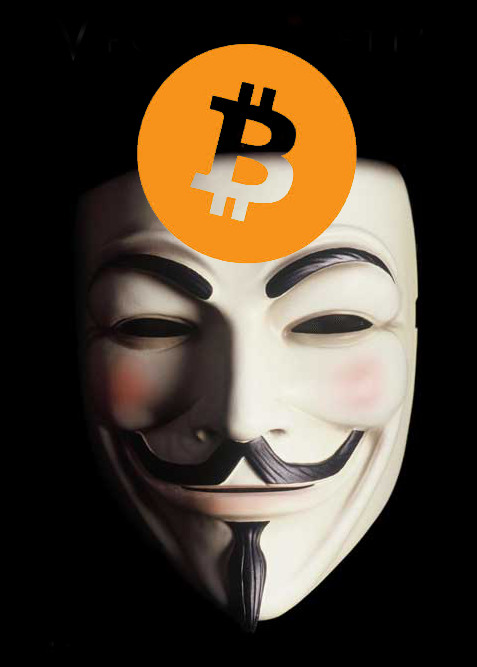
\includegraphics{vbitcoin.jpg}}

\captionsetup[floatingfigure]{labelformat=empty}
\begin{floatingfigure}[l]{0.24\textwidth}
\centering
\href{http://bakerjd99.wordpress.com/2014/02/08/bitcoin-is-a-perfect-protest/vbitcoin/}{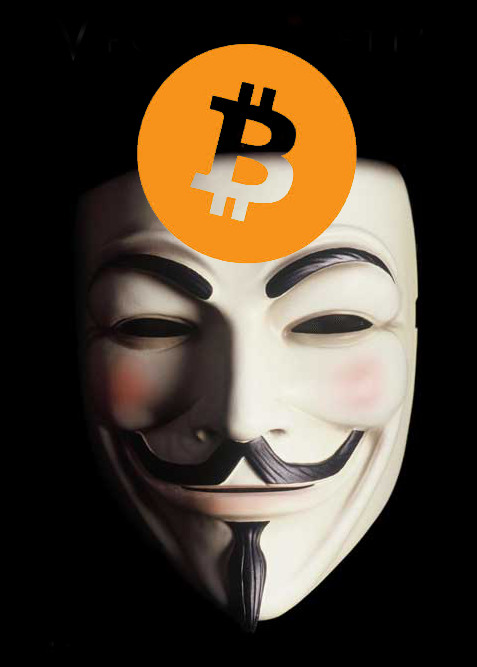
\includegraphics[width=0.22\textwidth]{vbitcoin.jpg}}
\label{fig:4521X0}
\end{floatingfigure} The
most intelligent comment I have read about
\href{https://bitcoin.org/en/}{Bitcoin} is that it's a \emph{perfect
protest}. \href{https://en.bitcoin.it/wiki/Genesis_block}{Bitcoin went
live in 2009} shortly after the 2008 financial crisis. The 2008 crisis
was a defining moment. Prior to that date I \emph{believed} that the US
government, despite its obvious warts, short comings and long checkered
history was still \emph{partly accountable} to the electorate. I didn't
buy the widespread cynical notion that modern elections are largely
meaningless dog and pony shows that help sell the illusion that
\emph{the people} are in charge. I seriously thought there were
important differences between Barak Obama, Hillary Clinton and John
McCain.~It's embarrassing to confess such naivety.

Before 2008 I was a good little cog in the machine: obediently paying my
taxes and being a productive member of society. I was a chump: a silly
stupid chump, but lucky for me, the
``\href{http://www.cbsnews.com/news/boehner-calls-bill-a-crap-sandwich-but-hell-vote-for-it/}{crap
sandwich}'' bank bailout cured my naivety. Despite being overwhelmingly
rejected by the public and initially rejected by Congress the crap
sandwich was forced down our throats and \emph{all three presidential
contenders voted for it.}  When push came to shove there were no
significant differences between liberal democrats and conservative
republicans, both groups lined up to betray and indebt the public and
we've been suffering, and will continue to suffer, the consequences for
years to come.

The 2008 financial crisis, and the comical US election that followed it,
taught me some important lessons:

\begin{enumerate}
%\itemsep1pt\parskip0pt\parsep0pt
\item
  \textbf{If none of the above is not on the ballot the election
  is fraudulent.} The political systems in the countries I have
  lived in depend on presenting limited, and frankly insulting choices,
  to the electorate. If anyone is going to seriously argue that Barak
  Obama and John McCain were the best that a country of three hundred
  million souls could offer then we are lost. If I was lost in the woods
  with Obama and McCain I wouldn't take a millisecond of direction from
  either and might consider getting rid of them on the spot to improve
  my chances of survival. A candidate must be better than nothing, and
  if nothing is superior to the highly gamed political selections put
  forward then nothing should be on the ballot! I will return to this
  theme in future posts. The next time you cast a ballot look for none
  of the above. If none of the above is not present the election is
  illegitimate and you are being used to put a stamp of public approval
  on what's very probably a vacuous choice.
\item
  \textbf{You can tell we're dealing with a real issue when the
  ruling class closes ranks.} Our idiotic media maelstrom is
  inconsequential noise that is best ignored. Will a society with gay
  marriage manage their finances better than a society without gay
  marriage? Will free birth control pills for sluts impact trade
  balances? Will crosses on public lands constrain money creation? Does
  the size of Kim Kardashian's ass moderate capital controls? Get in
  the habit of asking such questions. If the question is absurd, or if
  the answer doesn't matter, it's a distraction. On the other hand if
  you see alleged ideological enemies coming together to promote a
  \emph{critical common good} beware! In 2008 the flamboyant cosmetic
  differences between liberals and conservatives vanished removing even
  the illusion of choice. To bailout, or not bailout, was a real issue
  and with real issues there is no choice. We've recently witnessed rank
  closing on Edward Snowden. Again, both left-wing democrats and
  right-wing republicans lined up to declare Snowden a traitor and
  praise the glories of our NSA surveillance state. Clearly public
  privacy is another real issue and with real issues there is~no choice.
\item
  \textbf{Human beings cannot be trusted with money
  creation.} The 2008 bank bailout was outrageous for two
  primary reasons. It lavishly rewarded bad behavior and it created
  money to do it. Money creation~is convoluted; many argue that
  commercial banks create the bulk of money through loans, others claim
  the Federal Reserve creates money when buying government bonds and
  treasuries. The food chain is twisted but nobody disputes that
  \emph{at the base of the chain money is created out of nothing.}
  Everything boils down to ledger entries made by sanctioned
  authorities. There is no mining, there is no collateral, there's
  nothing but an invisible yoke that's \emph{eventually} placed on the
  public's head. The invisible yoke has briefly shown itself in the
  fiery debt limit fights about the \emph{full faith and credit of the
  United States.} What the hell is the full faith and credit of the
  United States? It's nothing more than a promise that the government
  will somehow extract the means to make payments to that long forgotten
  ledger entry. If the public fully understood that their labor is
  balanced against \emph{nothing} they would refuse to pay and the
  entire system would collapse. The system is such a perfect scam it's
  hard not to admire it. Oh, it will eventually collapse;
  \href{http://dailyreckoning.com/fiat-currency/}{fiat money always goes
  to zero}, but in the meanwhile, it affords unlimited fiscal
  flexibility to the ruling class. Who gets to create money is a real
  issue and once again there is~no choice about real issues.
\end{enumerate}

There has been a lot of nonsense written about Bitcoin but one thing is
clear it serves as a brilliant financial foil~so I am not surprised to
see recent worldwide
\href{http://www.coindesk.com/btce-pulls-support-ruble-russia-bans-bitcoin/}{efforts
to suppress it}. The most frightening thing about Bitcoin is that it
gets people asking questions about money. For example:

\begin{enumerate}
%\itemsep1pt\parskip0pt\parsep0pt
\item
  \textbf{Exactly what is money?} Every crank has their own
  definition of money. What amuses me is that both Gold cranks and fiat
  cranks have lambasted Bitcoin for being arbitrary and made up. One of
  the best retorts to this confused drivel notes that Bitcoin is to
  ``real money'' like the \href{http://www.venganza.org/}{Flying
  Spaghetti Monster} is to ``real religion.'' Everyone sees the Flying
  Spaghetti Monster is made up, but -- oddly -- nobody can mount
  rational arguments explaining why it's \emph{more made up} than the
  ``real thing.'' Bitcoin is capable of playing the \emph{role of
  money,} so in proper contexts it is money.
\item
  \textbf{Why do banking authorities have exclusive money creation
  rights}? The historic \emph{rationale} was to prevent counterfeiting.
  Counterfeiting is irresistible to anyone in a position to do it. By
  giving money creation rights to select authorities and using deadly
  force on counterfeiters governments could claim they were protecting
  the ``currency of the realm.'' It is many orders of magnitude more
  difficult to counterfeit Bitcoins than US dollars or any national
  currency. To counterfeit a Bitcoin you have to break a hard
  cryptographic hash. Technology has rendered the rationale for central
  money creation authorities obsolete.
\item
  \textbf{Should money be created without limit from nothing?} Now that
  monetary creation restraints, historically ties to gold, no longer
  exist~the only limit on creating money out of nothing is the stupidity
  of the public. How much debt can you get poor dumb suckers to accept
  before they rebel? Bitcoins are not created out of nothing. The mining
  process validates the public ledger, the Blockchain, and insures that
  nobody is counterfeiting coins or double spending. Mined coins are a
  reward for valuable network services. Additionally, there is no
  central creation authority. Competing miners create~Bitcoins
  all over the world. This system is not without fault and
  \href{http://vertcoin.org/}{Bitcoin variants} are exploring technical
  improvements but the Bitcoin creation process is essentially a
  mathematically secured network phenomenon and it is much harder to
  corrupt than bribing a few central bankers.
\item
  \textbf{Why do authorities maintain the right to confiscate private
  funds?} A Bitcoin feature that is particularly disturbing to
  authorities is that it's not difficult to prevent even powerful
  entities from seizing coins. A coin cannot be moved or spent unless
  you get its private key. If you do not know the private key a Bitcoin
  will just sit in the Blockchain taunting goons that covet it. In a
  Bitcoin economy it will be difficult to garnish wages, block money
  transfers and seize assets. How will the state survive?
\item
  \textbf{Why must fees be levied when moving money across national
  borders?} The public has never accepted this little rape. How many of
  us have lied to custom officials when asked about how much cash we're
  carrying?  I'm guessing a fair fraction of all travelers. We all know
  it's none of their damn business but being good little cogs we bend
  over and submit to state sodomy. Bitcoin penetrates borders with the
  same ease that custom authorities conduct cavity searches. Go ahead
  cut off coin movement! All you have to do is turn off the Internet,
  commander all USB ports, block old fashioned paper mail and learn how
  to read people's minds. Any information storage and transmission
  device, including the human brain, can be used to move coins. Go fuck
  yourself customs. One day money will be free to move without your
  permission or consent!
\end{enumerate}

Obviously we cannot have too many people asking such questions.
Mathematically sound, open source, publicly validated and distributed
real money like Bitcoin must be ridiculed, harassed and stopped. Left
unchecked it will cauterize an important component of state power:
arbitrary money creation rights. By providing an elegant mathematical
model of how a world without central banking and national currencies
might function Bitcoin is a perfect protest: a good idea that our
corrupt ``leaders'' cannot honestly answer.

%\captionsetup[floatingfigure]{labelformat=empty}
%\begin{figure}[htbp]
%\begin{floatingfigure}[l]{0.25\textwidth}
%\centering
%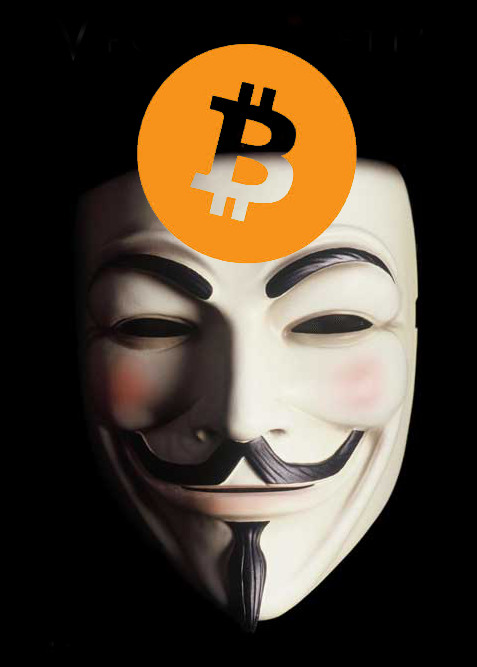
\includegraphics[width=0.23\textwidth]{vbitcoin.jpg}
%\caption{~~~IMCAPTION~~~}
%\label{fig:4521X0}
%\end{floatingfigure}
%\end{figure}


%\end{document}